\documentclass{article}
\usepackage{graphicx} % Required for inserting images
\usepackage{geometry}
\usepackage{cite}
\usepackage{multicol}
\geometry{hmargin=2.5cm,vmargin=1.5cm}


\title{Agent-based model of nest-site selection in a mass-recruiting ant \cite{agent_based_model}}
\author{Meggy Lie Anne  Chamand, Clara Stavun, Bella Muradian and Kim Georget}

\date{November 19, 2023}

\begin{document}

\maketitle


\textbf{This study investigates collective decision-making in ant nest-site selection, focusing on the M. nipponica ant's emigration process. Using an agent-based model in NetLogo, the research explores the significance of various parameters in decision-making, including environmental, ant-related, and physical factors. The model incorporates key mechanisms such as pheromone trails, quorum thresholds, and individual-level parameters. Results validate the model's accuracy, revealing insights into the trade-off between decision speed and accuracy, the impact of individual acceptance thresholds, and the adaptability of ants' decision strategies to environmental complexity. Future enhancements include introducing parameters for nest site quality, individual differences, and environmental factors to explore unexplored aspects of ant collective decision-making.}

\section{Introduction}
\subsection{Overview of the problem}
Ants, with their self-organizational prowess, captivate researchers in architecture construction and decision-making. Social insects, especially ants, offer an ideal study due to their simple yet intriguing individuals observable in labs, capable of remarkable feats. By deciphering how ants function and understanding the reasons behind their behaviors, we can apply these insights in various fields, including robotics. Despite knowledge of ant colony methods, many aspects, including environmental perception and behavioral rules, remain unknown. Hence, models are developed to explore the significance of different parameters, aiming to create realistic representations.\\
In our specific case, we delve into the nest emigration process of the M. nipponica ant, which utilizes chemical traces (pheromones) and a quorum-based decision-making process (a quorum is the minimum number of ants required for a nest site to be deemed viable) \cite{key_consensus_decision}. However, uncertainties persist regarding the extent of influence exerted by the various parameters such as the pheromone trails on ant movements for instance. Therefore, through this project, we aim to address this problem: \textbf{What is the significance of various parameters (environmental, ant-related, and physical parameters) in collective decision-making?}\\
The objectives of this study include replicating mass recruiting, clarifying individual parameters' significance, assessing heterogeneity importance, and investigating key parameters' impact on decision-making speed and accuracy.
 

\subsection{Existing models}
Various models elucidate how ants collectively decide on nest-site selection, with key ones being:\\
\textbf{Quorum Sensing}: Ants employ a quorum-sensing mechanism, depositing pheromones at potential nest sites. In this model, site selection depends on the cumulative pheromone threshold, aligning with observed ant behavior.\cite{quorum_sensing_recruitment}\\
\textbf{Heterogeneous Acceptance Thresholds}: Ants exhibit diverse acceptance thresholds for nest sites. In this model, thresholds determine the minimum pheromone level required for acceptance, influencing the speed and precision of decision-making. \cite{computational_model}\\
\textbf{Variable Individual Assessment Behavior}: Ants differ in their assessment behavior, some favoring proximity to food sources, while others prioritize concealment from predators. This model accommodates various empirical observations of ant nest-site selection. \cite{variability_individual_assessment}\\\\
Despite these models, limitations arise from their focus on specific parameters, hindering the identification of their relative influence. To overcome this, our approach incorporates multiple parameters, assessing their importance through varied values.

 

\section{Method}
\subsection{Tools}

To solve the problem written above, we will use an agent-based model built in NetLogo.
NetLogo is a widely used agent-based modeling environment tailored for simulating complex systems. It provides a user-friendly platform for creating models where individual agents, in this case, ants, interact within a collective. NetLogo's design simplifies the representation of intricate behaviors, allowing researchers to explore and analyze social dynamics effectively. With its visual interface, users can observe real-time simulations, making it even more suitable for studying ant social behavior, in particular collective decision-making.

\subsection{Model}

To replicate the process of nest-site selection by ants, our model will include as many components of the system as possible.
As mentioned before, this ant species relies on pheromone trails for navigation and also for the mechanism of recruitment. Combined with the use of quorum thresholds, this ‘voting’ via pheromone trails forms the primary mechanism for effecting collective decisions. 

 
\subsubsection{Agent parameters}
The study focused on small ant colonies comprising 10-70 ants. Agents adhered to a simple algorithm driven by individual-level parameters, with group-level properties emerging from agent interactions.

Four agent types were identified:

\begin{itemize}
    \item Nest ants: Remain in the original nest until transitioning to scouts based on a scout parameter.
    \item Scout ants: Explore the area randomly or follow pheromone trails, accepting candidate nests above an internal threshold.
    \item Decided ants: Lay pheromone trails between nests, committing at a rate determined by the commitment parameter.
    \item Transport ants: Move between chosen and original nests, transporting brood until relocation is complete.
\end{itemize}
The model's ant parameters set threshold levels for social and environmental signals, influencing behavior:

Wait: Time spent in new sites

Scout: Likelihood of becoming a scout

Accept: Threshold for accepting a site

Accept SD: Standard deviation for the normal distribution of Accept values

Quorum: Threshold number of ants in a new site to switch to transporting

Accept distribution: Distribution used for generating Accept thresholds

Commitment: Rate at which committed ants remain committed

Trail: Rate at which trails are followed if present


\subsubsection{Environment setup}
During nest emigration, ants undergo a three-phase process: the search phase, where candidate nests are located; the assessment phase, culminating in a quorum decision at a site; and the transport phase, concluding with the complete relocation of the nest.\\
The environment is a 101x101 unit square chamber, with the source nest at the center. New nests, arranged in balanced patterns, are located 38 units from the center, with variations in quality (good or poor) and random assignment of the single good nest among candidate sites.\\
Emigration has a fixed time limit of 15,000 steps, approximately five times the average successful immigration time for average-size colonies in simulations with base parameters. Success is defined as emigrating to the best available nest, split if items are transported to multiple nests, and failure if ants move to a lower-quality nest or don't complete emigration within the time limit.\\
Simulations will run for multiple replicates, varying parameter values from a base setting to test different configurations.


\subsection{Way of proceeding}
We plan on conducting simulations with replicates, exploring different parameter values to comprehend the nuances of the decision-making process in ant nest-site selection.


\section{Results}
\subsection{Model visualisation}

\begin{figure}[h]
    \centering
    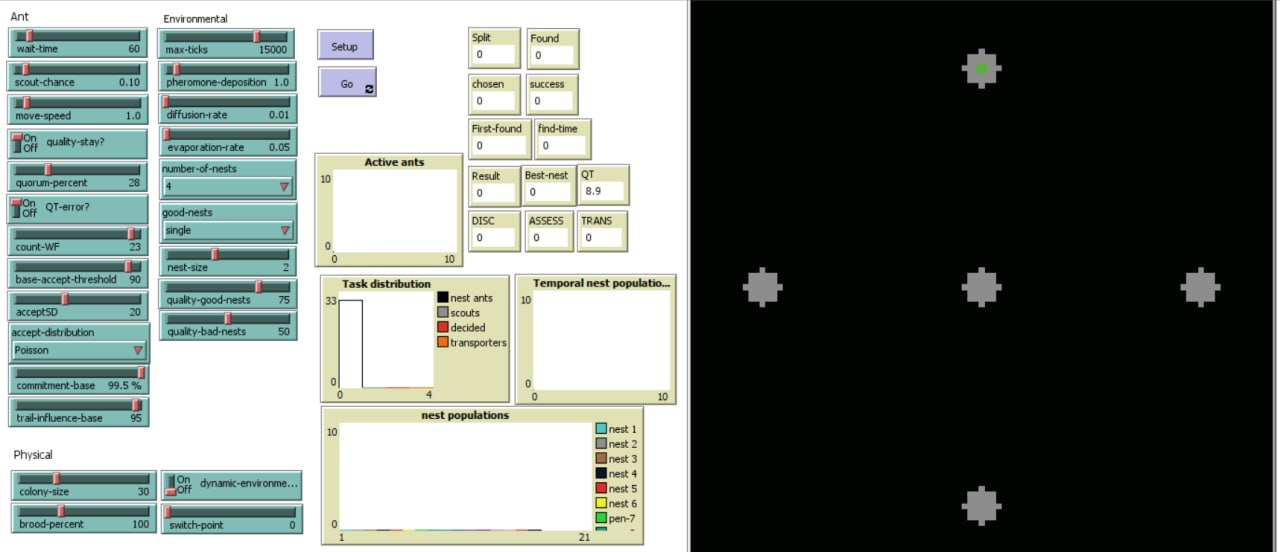
\includegraphics[width=0.65\textwidth]{Images/im1.jpeg}
    \caption{Environment setup for simulation in NetLogo with 4 possible nests}
    \label{fig:b11}
\end{figure}

All the parameters discussed in the part “Method” can be modified.
In this setup, the original nest is positioned in the middle, while all the potential nests are located at an equal distance from it, and the best nest is represented with a green dot. 

For the search phase, during which the ants are looking for a suitable new nest (Figure \ref{fig:b12})
\begin{figure}[h]
    \centering
    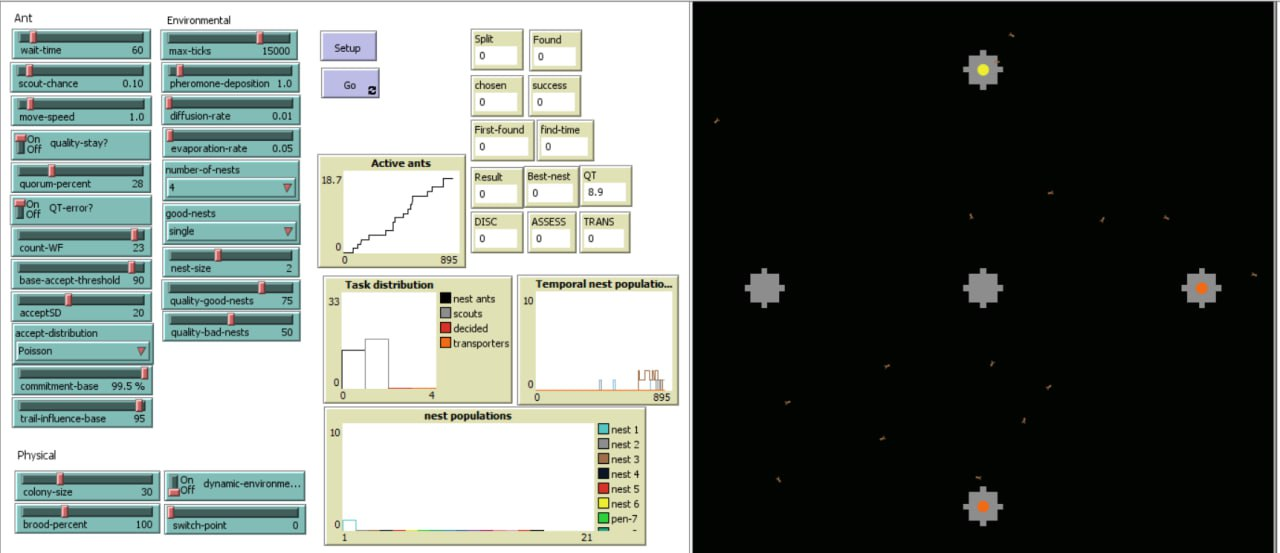
\includegraphics[width=0.65\textwidth]{Images/im2.jpeg}
    \caption{Model during the search phase}
    \label{fig:b12}
\end{figure}
Once a suitable nest has been found the ants move from their original nest: that’s the transport phase (Figure \ref{fig:b13}).

\begin{figure}[h]
    \centering
    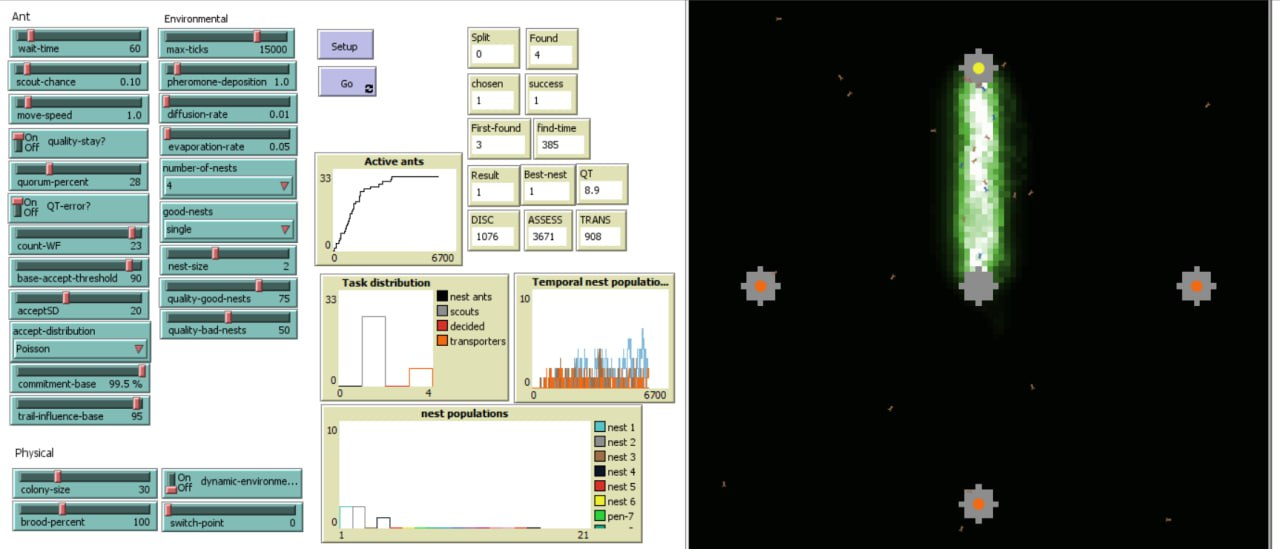
\includegraphics[width=0.65\textwidth]{Images/im3.jpeg}
    \caption{Model during the transport phase}
    \label{fig:b13}
\end{figure}

The white/green trails correspond to pheromones.
\\

\subsection{Paper results}
Firstly, the model undergoes validation as an accurate representation of the natural system, successfully reproducing the time course of nest-site selection for the ant species in question.\\
The model's outcomes also align with prior studies, highlighting the necessity of both social and private information for effective nest-site selection. Social information, such as pheromone trails, aids in identifying potential nest sites, while private information, reflecting individual preferences, plays a crucial role in evaluating site suitability.\\
Moreover, the model demonstrates that even a small number of individuals capable of distinguishing between good and bad nest sites can significantly impact collective decision-making.\\
Furthermore, the model reveals that the trade-off between speed and accuracy in nest-site selection is influenced by individual acceptance thresholds rather than quorum ones. Ants with lower acceptance thresholds are prone to swiftly accepting a nest site, while those with higher thresholds take more time for an informed decision, potentially delaying the selection process.\\
Lastly, the model indicates that ants can adapt their acceptance thresholds to the complexity of the environment, maximizing the success of nest-site selection. In complex environments, ants tend to be more selective, while in less complex ones, they can afford to be less selective and make quicker decisions.

 


\section{Discussion}
In summary, this agent-based model simulates ant nest-site selection, encompassing vital factors like pheromone trails, quorum thresholds, and individual parameters. The visualized emigration phases vividly depict ant behavior during exploration, assessment, and relocation. Findings affirm the model's accuracy, underscoring the importance of social and private information in decision-making. Notably, the study reveals how individual acceptance thresholds impact the balance between decision speed and accuracy, and it unveils the adaptability of ants' thresholds to environmental complexity, offering insights into dynamic strategies in collective decision-making within ant colonies.\\
\\
While the current model is comprehensive, we aim to broaden its scope by introducing additional parameters to delve into unexplored aspects.\\
One aspect we'll explore is the impact of nest site quality on decision-making, addressing the current model's oversight of variations in shelter, resource access, and exposure to environmental elements. By introducing a parameter for nest site quality, we'll assess how these variations influence decision-making.\\
Similarly, the model currently overlooks individual differences in ant preferences for nest sites. We plan to address this by introducing a parameter for individual differences, examining how diverse ant preferences contribute to decision-making, and considering factors like proximity to food sources or predator avoidance.\\
Additionally, the model doesn't currently consider the influence of environmental factors on nest site selection. Our strategy involves introducing parameters for environmental factors to investigate their impact on decision-making.

 
\bibliographystyle{plain}
\bibliography{bib/bibliography}



\end{document}
